
%% Test of Understandin of vectors: A reliable multiple-choice vector concept test
%% Pablo Barniol and Genearo Zavala
%% Phys. Rev. ST Phys. Educ. Res. 10, 010121--Published 17 June 2014


%% Test of Understanding Vectors
%%--------------------------------------------------
\element{vectors}{
\begin{question}{vectors-q01}
    The figure below shows vectors $\vec{\mathbf{A}}$ and $\vec{\mathbf{B}}$.
    \begin{center}
    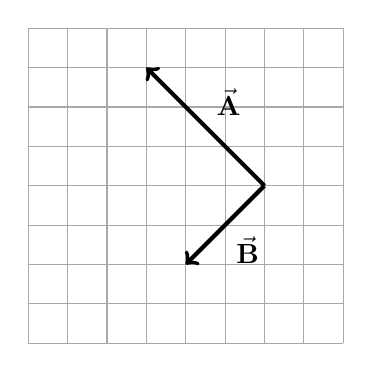
\begin{tikzpicture}
        \draw[white!66!black,step=0.50cm] (0,0) grid (4,4);
        \draw[line width=1.5pt,->] (3,2) -- ++(-1.5,1.5) node[pos=0.5,anchor=south west] {$\vec{\mathbf{A}}$};
        \draw[line width=1.5pt,->] (3,2) -- ++(-1,-1) node[pos=0.5,anchor=north west] {$\vec{\mathbf{B}}$};
    \end{tikzpicture}
    \end{center}
    Choose the option that shows the vector sum 
        $\vec{\mathbf{A}} + \vec{\mathbf{B}}$.
    \begin{multicols}{2}
    \begin{choices}
        \AMCboxDimensions{down=-1.5cm}
        \wrongchoice{
            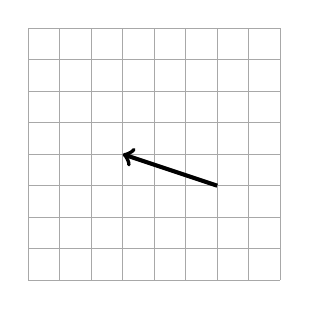
\begin{tikzpicture}[scale=0.8]
                \draw[white!66!black,step=0.50cm] (0,0) grid (4,4);
                \draw[line width=1.5pt,->] (3,1.5) -- ++(-1.5,0.5);
            \end{tikzpicture}
        }
        \wrongchoice{
            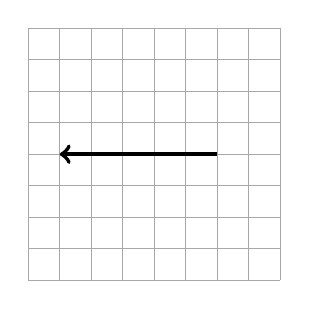
\begin{tikzpicture}[scale=0.8]
                \draw[white!66!black,step=0.50cm] (0,0) grid (4,4);
                \draw[line width=1.5pt,->] (3,2) -- ++(-2.5,0);
            \end{tikzpicture}
        }
        \wrongchoice{
            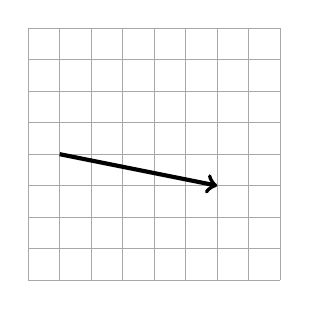
\begin{tikzpicture}[scale=0.8]
                \draw[white!66!black,step=0.50cm] (0,0) grid (4,4);
                \draw[line width=1.5pt,->] (0.5,2) -- ++(2.5,-0.5);
            \end{tikzpicture}
        }
        \wrongchoice{
            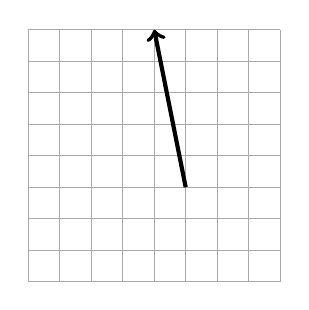
\begin{tikzpicture}[scale=0.8]
                \draw[white!66!black,step=0.50cm] (0,0) grid (4,4);
                \draw[line width=1.5pt,->] (2.5,1.5) -- ++(-0.5,2.5);
            \end{tikzpicture}
        }
        \correctchoice{
            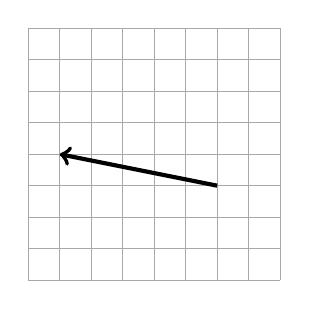
\begin{tikzpicture}[scale=0.8]
                \draw[white!66!black,step=0.50cm] (0,0) grid (4,4);
                \draw[line width=1.5pt,->] (3,1.5) -- ++(-2.5,0.5);
            \end{tikzpicture}
        }
        %% NOTE: six for symmetry
    \end{choices}
    \end{multicols}
\end{question}
}

\element{vectors}{
\begin{question}{vectors-q02}
    The figure below shows vector $\vec{\mathbf{A}}$.
    \begin{center}
    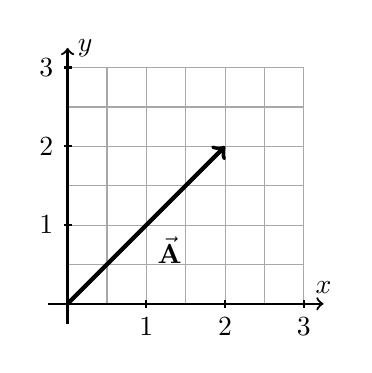
\begin{tikzpicture}
        \draw[white] (-0.5,-0.5) rectangle (3.5,3.5);
        \draw[white!66!black,step=0.5cm] (0,0) grid (3,3);
        \draw[thick,->] (-0.25,0) -- (3.25,0) node[anchor=south] {$x$};
        \draw[thick,->] (0,-0.25) -- (0,3.25) node[anchor=west] {$y$};
        \foreach \i in {1,2,3}{
            \draw[thick] (0.05,\i) -- (-0.05,\i) node[anchor=east] {$\i$};
            \draw[thick] (\i,0.05) -- (\i,-0.05) node[anchor=north] {$\i$};
        }
        \draw[line width=1.5pt,->] (0,0) -- (2,2) node[pos=0.5,anchor=north west] {$\vec{\mathbf{A}}$};
    \end{tikzpicture}
    \end{center}
    Choose the option that shows the unit vector in the direction of vector $\vec{\mathbf{A}}$.
    \begin{multicols}{2}
    \begin{choices}
        \AMCboxDimensions{down=-1.25cm}
        \wrongchoice{
            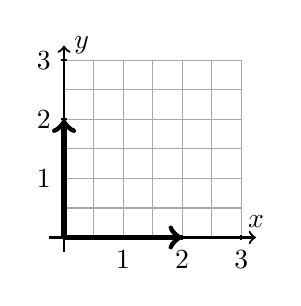
\begin{tikzpicture}[scale=0.75]
                \draw[white] (-0.5,-0.5) rectangle (3.5,3.5);
                \draw[white!66!black,step=0.5cm] (0,0) grid (3,3);
                \draw[thick,->] (-0.25,0) -- (3.25,0) node[anchor=south] {$x$};
                \draw[thick,->] (0,-0.25) -- (0,3.25) node[anchor=west] {$y$};
                \foreach \i in {1,2,3}{
                    \draw[thick] (0.05,\i) -- (-0.05,\i) node[anchor=east] {$\i$};
                    \draw[thick] (\i,0.05) -- (\i,-0.05) node[anchor=north] {$\i$};
                }
                \draw[line width=2.0pt,->] (0,0) -- (0,2);
                \draw[line width=2.0pt,->] (0,0) -- (2,0);
            \end{tikzpicture}
        }
        \wrongchoice{
            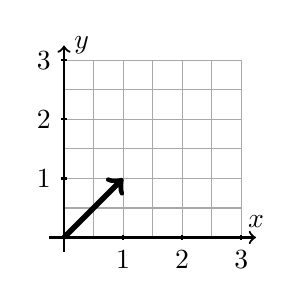
\begin{tikzpicture}[scale=0.75]
                \draw[white] (-0.5,-0.5) rectangle (3.5,3.5);
                \draw[white!66!black,step=0.5cm] (0,0) grid (3,3);
                \draw[thick,->] (-0.25,0) -- (3.25,0) node[anchor=south] {$x$};
                \draw[thick,->] (0,-0.25) -- (0,3.25) node[anchor=west] {$y$};
                \foreach \i in {1,2,3}{
                    \draw[thick] (0.05,\i) -- (-0.05,\i) node[anchor=east] {$\i$};
                    \draw[thick] (\i,0.05) -- (\i,-0.05) node[anchor=north] {$\i$};
                }
                \draw[line width=2.0pt,->] (0,0) -- (1,1);
            \end{tikzpicture}
        }
        %% ANS unit vector has length 1
        \correctchoice{
            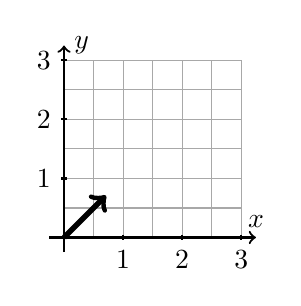
\begin{tikzpicture}[scale=0.75]
                \draw[white] (-0.5,-0.5) rectangle (3.5,3.5);
                \draw[white!66!black,step=0.5cm] (0,0) grid (3,3);
                \draw[thick,->] (-0.25,0) -- (3.25,0) node[anchor=south] {$x$};
                \draw[thick,->] (0,-0.25) -- (0,3.25) node[anchor=west] {$y$};
                \foreach \i in {1,2,3}{
                    \draw[thick] (0.05,\i) -- (-0.05,\i) node[anchor=east] {$\i$};
                    \draw[thick] (\i,0.05) -- (\i,-0.05) node[anchor=north] {$\i$};
                }
                \draw[line width=2.0pt,->] (0,0) -- (0.71,0.71);
            \end{tikzpicture}
        }
        \wrongchoice{
            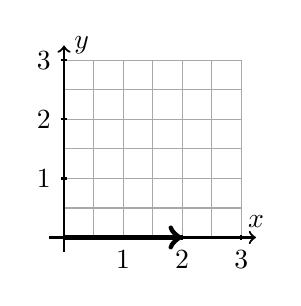
\begin{tikzpicture}[scale=0.75]
                \draw[white] (-0.5,-0.5) rectangle (3.5,3.5);
                \draw[white!66!black,step=0.5cm] (0,0) grid (3,3);
                \draw[thick,->] (-0.25,0) -- (3.25,0) node[anchor=south] {$x$};
                \draw[thick,->] (0,-0.25) -- (0,3.25) node[anchor=west] {$y$};
                \foreach \i in {1,2,3}{
                    \draw[thick] (0.05,\i) -- (-0.05,\i) node[anchor=east] {$\i$};
                    \draw[thick] (\i,0.05) -- (\i,-0.05) node[anchor=north] {$\i$};
                }
                \draw[line width=2.0pt,->] (0,0) -- (2,0);
            \end{tikzpicture}
        }
        \wrongchoice{
            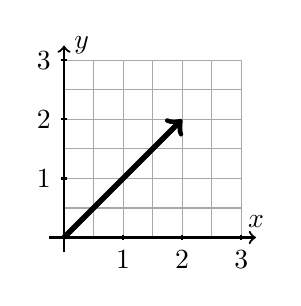
\begin{tikzpicture}[scale=0.75]
                \draw[white] (-0.5,-0.5) rectangle (3.5,3.5);
                \draw[white!66!black,step=0.5cm] (0,0) grid (3,3);
                \draw[thick,->] (-0.25,0) -- (3.25,0) node[anchor=south] {$x$};
                \draw[thick,->] (0,-0.25) -- (0,3.25) node[anchor=west] {$y$};
                \foreach \i in {1,2,3}{
                    \draw[thick] (0.05,\i) -- (-0.05,\i) node[anchor=east] {$\i$};
                    \draw[thick] (\i,0.05) -- (\i,-0.05) node[anchor=north] {$\i$};
                }
                \draw[line width=2.0pt,->] (0,0) -- (2,2);
            \end{tikzpicture}
        }
        %% NOTE: six for symmetry
    \end{choices}
    \end{multicols}
\end{question}
}

\element{vectors}{
\begin{question}{vectors-q03}
    The figure below shows a vector $\vec{\mathbf{C}}$ and $\vec{\mathbf{D}}$.
    \begin{center}
    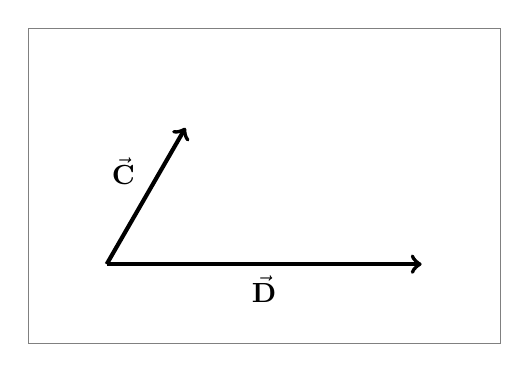
\begin{tikzpicture}
        \draw[help lines] ( -1,-1) rectangle (5,3);
        \draw[line width=1.5pt,->] (0,0) -- (60:2) node[pos=0.5,anchor=south east] {$\vec{\mathbf{C}}$};
        \draw[line width=1.5pt,->] (0,0) -- (0:4) node[pos=0.5,anchor=north] {$\vec{\mathbf{D}}$};
    \end{tikzpicture}
    \end{center}
    Which option is the best interpretation of the dot product $\vec{\mathbf{C}}\cdot\vec{\mathbf{D}}$?
    \begin{choices}
        \wrongchoice{The magnitude of a vector between $\vec{\mathbf{C}}$ and $\vec{\mathbf{D}}$ pointing up to the right.}
      \correctchoice{The projection of vector $\vec{\mathbf{C}}$ onto vector $\vec{\mathbf{D}}$ multplied by teh magnitude of vector $\vec{\mathbf{D}}$.}
        \wrongchoice{A vector between $\vec{\mathbf{C}}$ and $\vec{\mathbf{D}}$ pointing up to the right.}
        \wrongchoice{A vector perpendicular to both vectors.}
        \wrongchoice{A vector in the direction of $\vec{\mathbf{D}}$.}
    \end{choices}
\end{question}
}

\element{vectors}{
\begin{question}{vectors-q04}
    The figure below shows a vector $\vec{\mathbf{A}}$ that forms an angle $\phi$ with the vertical axis.
    \begin{center}
    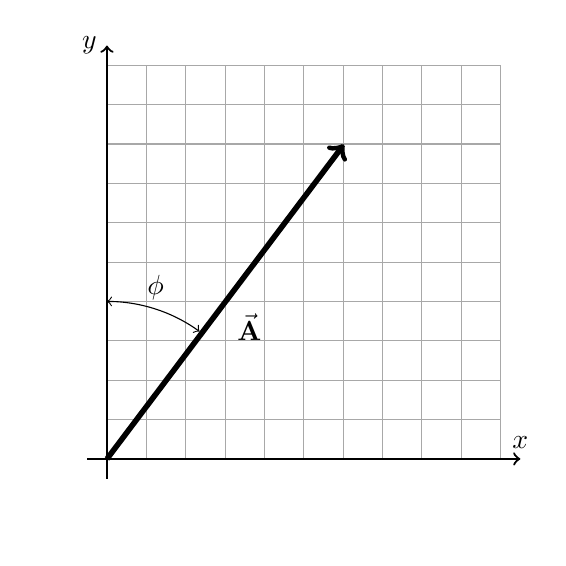
\begin{tikzpicture}
        \draw[white] (-1,-1) rectangle (4,5);
        \draw[white!66!black,step=0.5cm] (0,0) grid (5,5);
        \draw[thick,->] (-0.25,0) -- (5.25,0) node[anchor=south] {$x$};
        \draw[thick,->] (0,-0.25) -- (0,5.25) node[anchor=east] {$y$};
        \draw[line width=2pt,->] (0,0) -- (53:5) node[pos=0.5,anchor=north west] {$\vec{\mathbf{A}}$};
        \draw[<->] (0,2) arc (90:54:2) node[anchor=south,pos=0.5] {$\phi$};
    \end{tikzpicture}
    \end{center}
    Choose the option that shows the $y$-component vector of $\vec{\mathbf{A}}$, (\emph{i.e.} $\vec{\mathbf{A}}_y$).
    \begin{multicols}{2}
    \begin{choices}
        %% NOTE: mix x and y components in x and y direction
        \AMCboxDimensions{down=-1.25cm}
        \wrongchoice{
            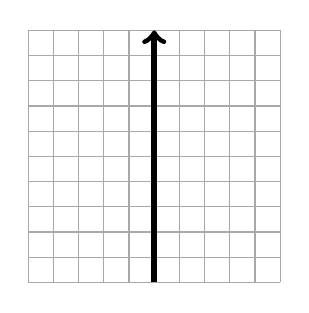
\begin{tikzpicture}[scale=0.64]
                \draw[white!66!black,step=0.5cm] (0,0) grid (5,5);
                \draw[line width=2pt,->] (2.5,0) -- ++(0,5);
            \end{tikzpicture}
        }
        \wrongchoice{
            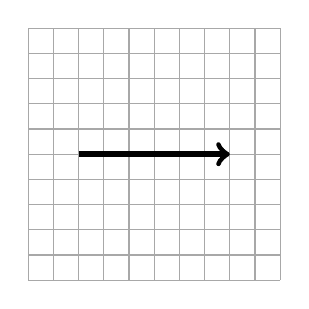
\begin{tikzpicture}[scale=0.64]
                \draw[white!66!black,step=0.5cm] (0,0) grid (5,5);
                \draw[line width=2pt,->] (1,2.5) -- ++(3,0);
            \end{tikzpicture}
        }
        \correctchoice{
            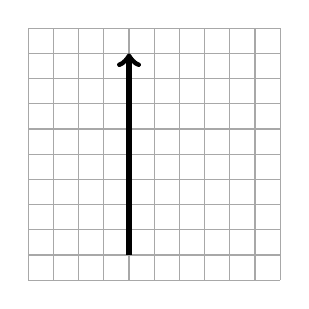
\begin{tikzpicture}[scale=0.64]
                \draw[white!66!black,step=0.5cm] (0,0) grid (5,5);
                \draw[line width=2pt,->] (2,0.5) -- ++(0,4);
            \end{tikzpicture}
        }
        \wrongchoice{
            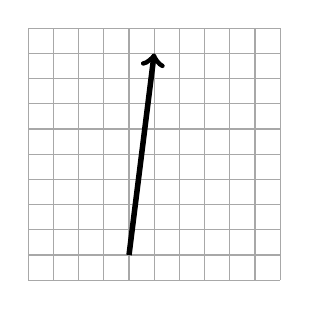
\begin{tikzpicture}[scale=0.64]
                \draw[white!66!black,step=0.5cm] (0,0) grid (5,5);
                \draw[line width=2pt,->] (2,0.5) -- ++(0.5,4);
            \end{tikzpicture}
        }
        \wrongchoice{
            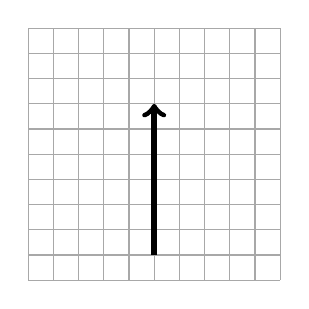
\begin{tikzpicture}[scale=0.64]
                \draw[white!66!black,step=0.5cm] (0,0) grid (5,5);
                \draw[line width=2pt,->] (2.5,0.5) -- ++(0,3);
            \end{tikzpicture}
        }
    \end{choices}
    \end{multicols}
\end{question}
}

\element{vectors}{
\begin{questionmult}{vectors-q05}
    The figure below shows vector $\vec{\mathbf{A}}$.
    \begin{center}
    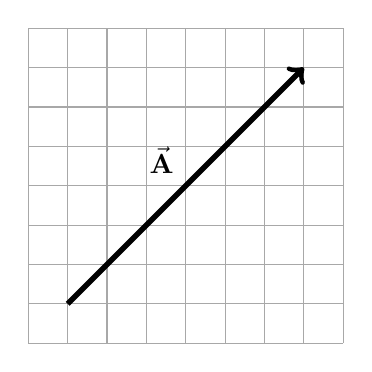
\begin{tikzpicture}
        \draw[white!66!black,step=0.5cm] (0,0) grid (4,4);
        \draw[line width=2pt,->] (0.5,0.5) -- ++(3,3) node[pos=0.5,anchor=south east] {$\vec{\mathbf{A}}$};
    \end{tikzpicture}
    \end{center}
    Which vector(s) has/have the same direction as vector $\vec{\mathbf{A}}$?
    \begin{multicols}{2}
    \begin{choices}
        \AMCboxDimensions{down=-1.5cm}
        %% option H
        \wrongchoice{
            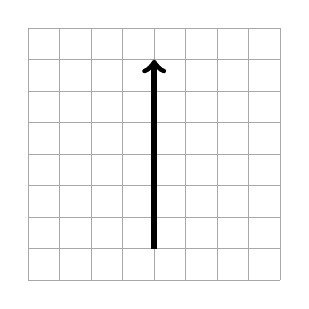
\begin{tikzpicture}[scale=0.8]
                \draw[white!66!black,step=0.5cm] (0,0) grid (4,4);
                \draw[line width=2pt,->] (2,0.5) -- (2,3.5);
            \end{tikzpicture}
        }
        %% option I
        \wrongchoice{
            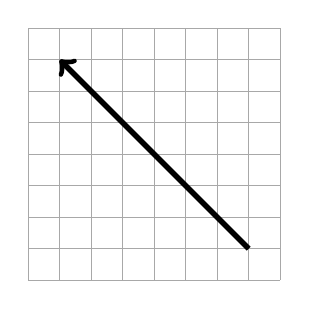
\begin{tikzpicture}[scale=0.8]
                \draw[white!66!black,step=0.5cm] (0,0) grid (4,4);
                \draw[line width=2pt,->] (3.5,0.5) -- (0.5,3.5);
            \end{tikzpicture}
        }
        %% option J
        \wrongchoice{
            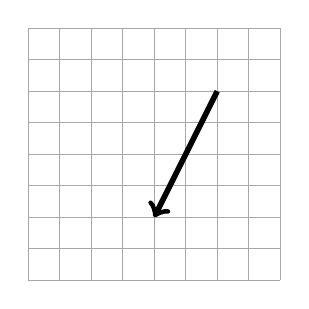
\begin{tikzpicture}[scale=0.8]
                \draw[white!66!black,step=0.5cm] (0,0) grid (4,4);
                \draw[line width=2pt,->] (3,3) -- ++(-1,-2);
            \end{tikzpicture}
        }
        %% option K
        \correctchoice{
            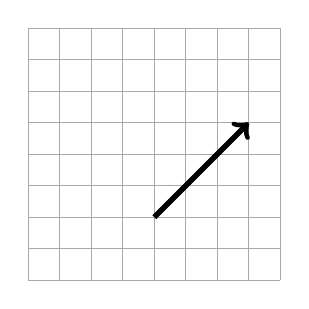
\begin{tikzpicture}[scale=0.8]
                \draw[white!66!black,step=0.5cm] (0,0) grid (4,4);
                \draw[line width=2pt,->] (2,1) -- ++(1.5,1.5);
            \end{tikzpicture}
        }
        %% option L
        \wrongchoice{
            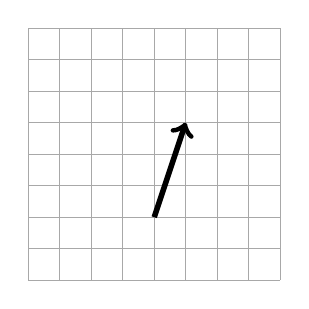
\begin{tikzpicture}[scale=0.8]
                \draw[white!66!black,step=0.5cm] (0,0) grid (4,4);
                \draw[line width=2pt,->] (2,1) -- ++(0.5,1.5);
            \end{tikzpicture}
        }
    \end{choices}
    \end{multicols}
\end{questionmult}
}

\element{vectors}{
\begin{question}{vectors-q06}
    The figure below shows vectors $\vec{\mathbf{A}}$ and $\vec{\mathbf{B}}$ that form an angle $\theta$.
    \begin{center}
    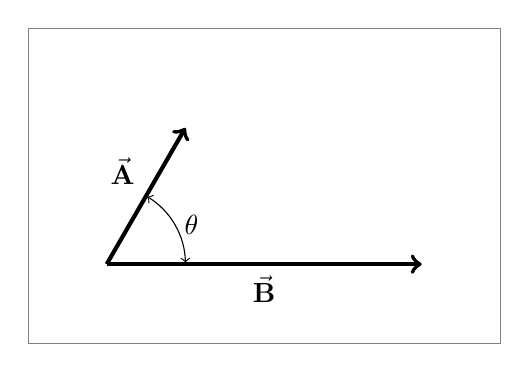
\begin{tikzpicture}
        \draw[help lines] (-1,-1) rectangle (5,3);
        \draw[line width=1.5pt,->] (0,0) -- (60:2) node[pos=0.5,anchor=south east] {$\vec{\mathbf{A}}$};
        \draw[line width=1.5pt,->] (0,0) -- (0:4) node[pos=0.5,anchor=north] {$\vec{\mathbf{B}}$};
        \draw[<->] (1:1) arc (1:59:1) node[pos=0.5,anchor=west] {$\theta$}; 
    \end{tikzpicture}
    \end{center}
    $\left|\vec{\mathbf{A}}\right|$ is the magnitude of vector $\vec{\mathbf{A}}$ and $\left|\vec{\mathbf{B}}\right|$ is the magnitude of vector $\vec{\mathbf{B}}$.
    Which option is the dot product $\left(\vec{\mathbf{A}}\cdot\vec{\mathbf{B}}\right)$?
    \begin{multicols}{2}
    \begin{choices}
        \wrongchoice{$\left|\vec{\mathbf{A}}\right| \left|\vec{\mathbf{B}}\right|$}
      \correctchoice{$\left|\vec{\mathbf{A}}\right| \left|\vec{\mathbf{B}}\right| \cos\theta$}
        \wrongchoice{$\left|\vec{\mathbf{A}}\right| \cos\theta + \left|\vec{\mathbf{B}}\right| \sin\theta$}
        \wrongchoice{$\left|\vec{\mathbf{A}}\right| \left|\vec{\mathbf{B}}\right| \sin\theta$}
        \wrongchoice{$\left|\vec{\mathbf{A}}\right| \cos\theta \left|\vec{\mathbf{B}}\right| \sin\theta$}
    \end{choices}
    \end{multicols}
\end{question}
}

\element{vectors}{
\begin{question}{vectors-q07}
    The figure below shows vectors $\vec{\mathbf{A}}$ and $\vec{\mathbf{B}}$ that have the same magnitude.
    \begin{center}
    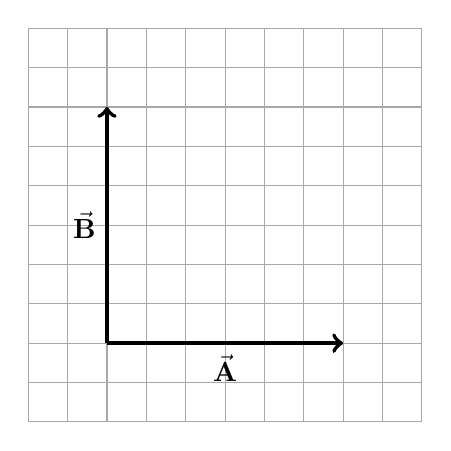
\begin{tikzpicture}
        \draw[white!66!black,step=0.5cm] (-1,-1) grid (4,4);
        \draw[line width=1.5pt,->] (0,0) -- (0:3) node[pos=0.5,anchor=north] {$\vec{\mathbf{A}}$};
        \draw[line width=1.5pt,->] (0,0) -- (90:3) node[pos=0.5,anchor=east] {$\vec{\mathbf{B}}$};
    \end{tikzpicture}
    \end{center}
    Which of the following statements about the magnitude of the vector sum of these two vectors is true?
    \begin{choices}
        \wrongchoice{The magnitude of the vector sum is equal to the magnitude of vector. The vector sum only changes direction.}
      \correctchoice{The magnitude of the vector sum is greater than the magnitude of vector, and it is demonstrated by the direct application of the Pythagorean theorem.}
        \wrongchoice{The magnitude of the vector sum is equal to the magnitude of vector, because vectors and have the same magnitude.}
        \wrongchoice{The magnitude of the vector sum is equal to the magnitude of vector, and it is demonstrated by the direct application of the Pythagorean theorem.}
        \wrongchoice{The magnitude of the vector sum is smaller than the magnitude of vector, because the two vectors are at a \ang{90} angle.}
    \end{choices}
\end{question}
}

\element{vectors}{
\begin{question}{vectors-q08}
    Consider the vector $\vec{\mathbf{A}} = 1\hat{\imath} + 3\hat{\jmath}$
        and $\vec{\mathbf{B}} = 5\hat{\imath}$.
    Which option is the dot product $\left(\vec{\mathbf{A}}\cdot\vec{\mathbf{B}}\right)$?
    \begin{multicols}{2}
    \begin{choices}
      \correctchoice{$5$}
        \wrongchoice{$-15\hat{k}$}
        \wrongchoice{$5\hat{\imath} + 3\hat{\jmath}$}
        \wrongchoice{$6\hat{\imath} + 3\hat{\jmath}$}
        \wrongchoice{$5\hat{\imath}$}
    \end{choices}
    \end{multicols}
\end{question}
}

\element{vectors}{
\begin{question}{vectors-q09}
    The figure below shows vectors $\vec{\mathbf{A}}$ that forms an angle $\phi$ with the vertcial axis.
    \begin{center}
    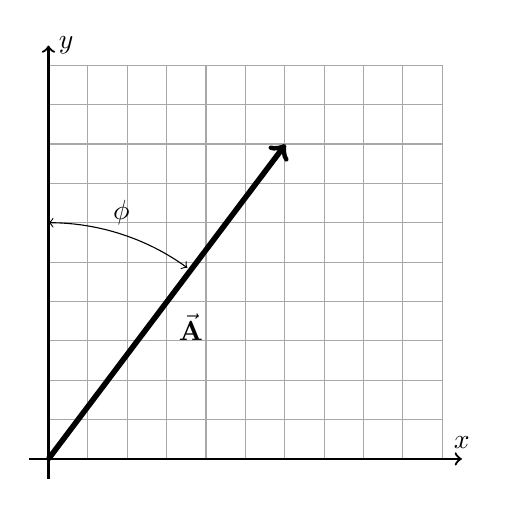
\begin{tikzpicture}
        %\draw[white] (-0.5,-0.2) rectangle (4.5,4.5);
        \draw[white!66!black,step=0.5cm] (0,0) grid (5,5);
        \draw[thick,->] (-0.25,0) -- (5.25,0) node[anchor=south] {$x$};
        \draw[thick,->] (0,-0.25) -- (0,5.25) node[anchor=west] {$y$};
        \draw[line width=2pt,->] (0,0) -- (53:5) node[pos=0.5,anchor=north west] {$\vec{\mathbf{A}}$};
        \draw[<->] (0,3) arc (90:54:3) node[anchor=south,pos=0.5] {$\phi$};
    \end{tikzpicture}
    \end{center}
    Choose the option that shows the $x$-component vector $\vec{\mathbf{A}}$ (\emph{i.e.} $\vec{\mathbf{A}_x}$).
    \begin{multicols}{2}
    \begin{choices}
        \AMCboxDimensions{down=-1.5cm}
        \correctchoice{
            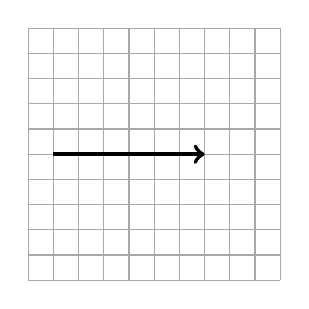
\begin{tikzpicture}[scale=0.64]
                \draw[white!66!black,step=0.5cm] (0,0) grid (5,5);
                \draw[line width=1.5pt,->] (0.5,2.5) -- ++(3,0);
            \end{tikzpicture}
        }
        \wrongchoice{
            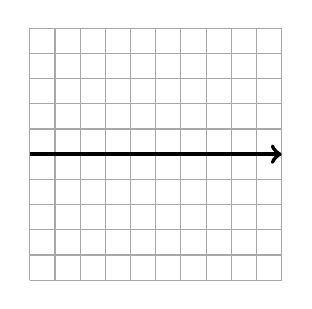
\begin{tikzpicture}[scale=0.64]
                \draw[white!66!black,step=0.5cm] (0,0) grid (5,5);
                \draw[line width=1.5pt,->] (0,2.5) -- ++(5,0);
            \end{tikzpicture}
        }
        \wrongchoice{
            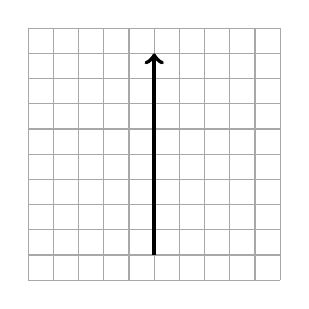
\begin{tikzpicture}[scale=0.64]
                \draw[white!66!black,step=0.5cm] (0,0) grid (5,5);
                \draw[line width=1.5pt,->] (2.5,0.5) -- ++(0,4);
            \end{tikzpicture}
        }
        \wrongchoice{
            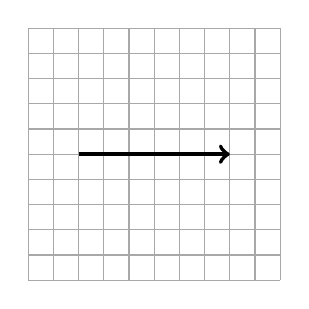
\begin{tikzpicture}[scale=0.64]
                \draw[white!66!black,step=0.5cm] (0,0) grid (5,5);
                \draw[line width=1.5pt,->] (1,2.5) -- ++(3,0);
            \end{tikzpicture}
        }
        \wrongchoice{
            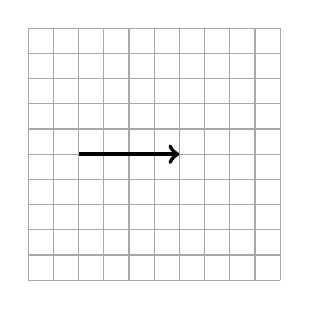
\begin{tikzpicture}[scale=0.64]
                \draw[white!66!black,step=0.5cm] (0,0) grid (5,5);
                \draw[line width=1.5pt,->] (1,2.5) -- ++(2,0);
            \end{tikzpicture}
        }
    \end{choices}
    \end{multicols}
\end{question}
}

\element{vectors}{
\begin{question}{vectors-q10}
    Choose the option that shows the vector $\vec{\mathbf{A}} = -2\hat{\imath} + 3\hat{\jmath}$.
    \begin{multicols}{2}
    \begin{choices}
        \AMCboxDimensions{down=-1.5cm}
        \wrongchoice{
            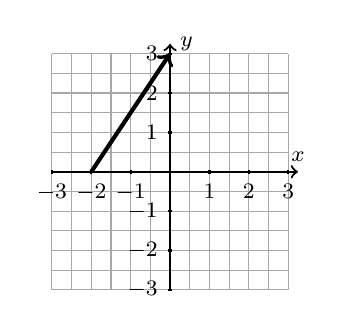
\begin{tikzpicture}[scale=0.5,font=\footnotesize]
                \draw[white!66!black,step=0.50cm] (-3,-3) grid (3,3);
                \draw[thick,->] (-3,0) -- (3.25,0) node[anchor=south] {$x$};
                \draw[thick,->] (0,-3) -- (0,3.25) node[anchor=west] {$y$};
                \foreach \i in {-3,-2,-1,1,2,3}{
                    \draw[thick] (0.05,\i) -- (-0.05,\i) node[anchor=east] {$\i$};
                    \draw[thick] (\i,0.05) -- (\i,-0.05) node[anchor=north] {$\i$};
                }
                \draw[line width=1.5pt,->] (-2,0) -- ++(2,3);
            \end{tikzpicture}
        }
        \correctchoice{
            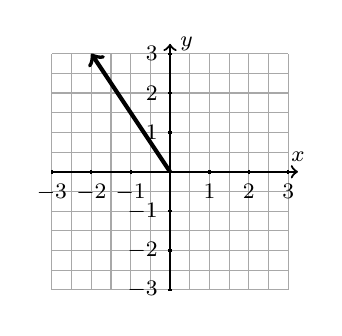
\begin{tikzpicture}[scale=0.5,font=\footnotesize]
                \draw[white!66!black,step=0.50cm] (-3,-3) grid (3,3);
                \draw[thick,->] (-3,0) -- (3.25,0) node[anchor=south] {$x$};
                \draw[thick,->] (0,-3) -- (0,3.25) node[anchor=west] {$y$};
                \foreach \i in {-3,-2,-1,1,2,3}{
                    \draw[thick] (0.05,\i) -- (-0.05,\i) node[anchor=east] {$\i$};
                    \draw[thick] (\i,0.05) -- (\i,-0.05) node[anchor=north] {$\i$};
                }
                \draw[line width=1.5pt,->] (0,0) -- ++(-2,3);
            \end{tikzpicture}
        }
        \wrongchoice{
            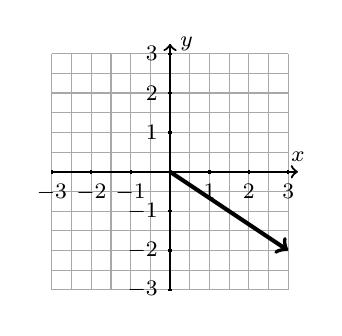
\begin{tikzpicture}[scale=0.5,font=\footnotesize]
                \draw[white!66!black,step=0.50cm] (-3,-3) grid (3,3);
                \draw[thick,->] (-3,0) -- (3.25,0) node[anchor=south] {$x$};
                \draw[thick,->] (0,-3) -- (0,3.25) node[anchor=west] {$y$};
                \foreach \i in {-3,-2,-1,1,2,3}{
                    \draw[thick] (0.05,\i) -- (-0.05,\i) node[anchor=east] {$\i$};
                    \draw[thick] (\i,0.05) -- (\i,-0.05) node[anchor=north] {$\i$};
                }
                \draw[line width=1.5pt,->] (0,0) -- ++(3,-2);
            \end{tikzpicture}
        }
        \wrongchoice{
            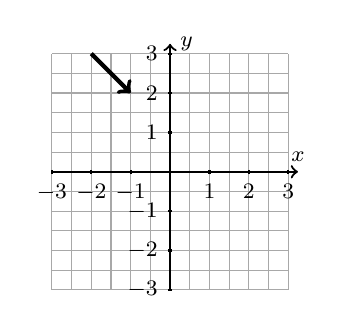
\begin{tikzpicture}[scale=0.5,font=\footnotesize]
                \draw[white!66!black,step=0.50cm] (-3,-3) grid (3,3);
                \draw[thick,->] (-3,0) -- (3.25,0) node[anchor=south] {$x$};
                \draw[thick,->] (0,-3) -- (0,3.25) node[anchor=west] {$y$};
                \foreach \i in {-3,-2,-1,1,2,3}{
                    \draw[thick] (0.05,\i) -- (-0.05,\i) node[anchor=east] {$\i$};
                    \draw[thick] (\i,0.05) -- (\i,-0.05) node[anchor=north] {$\i$};
                }
                \draw[line width=1.5pt,->] (-2,3) -- ++(1,-1);
            \end{tikzpicture}
        }
        \wrongchoice{
            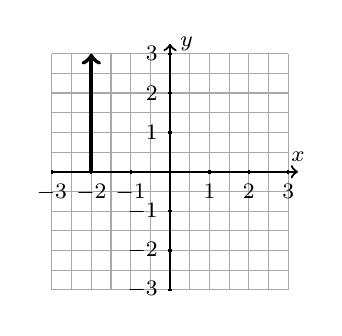
\begin{tikzpicture}[scale=0.5,font=\footnotesize]
                \draw[white!66!black,step=0.50cm] (-3,-3) grid (3,3);
                \draw[thick,->] (-3,0) -- (3.25,0) node[anchor=south] {$x$};
                \draw[thick,->] (0,-3) -- (0,3.25) node[anchor=west] {$y$};
                \foreach \i in {-3,-2,-1,1,2,3}{
                    \draw[thick] (0.05,\i) -- (-0.05,\i) node[anchor=east] {$\i$};
                    \draw[thick] (\i,0.05) -- (\i,-0.05) node[anchor=north] {$\i$};
                }
                \draw[line width=1.5pt,->] (-2,0) -- ++(0,3);
            \end{tikzpicture}
        }
    \end{choices}
    \end{multicols}
\end{question}
}

\element{vectors}{
\begin{question}{vectors-q11}
    The figure below shows vector $\vec{\mathbf{A}}$.
    \begin{center}
    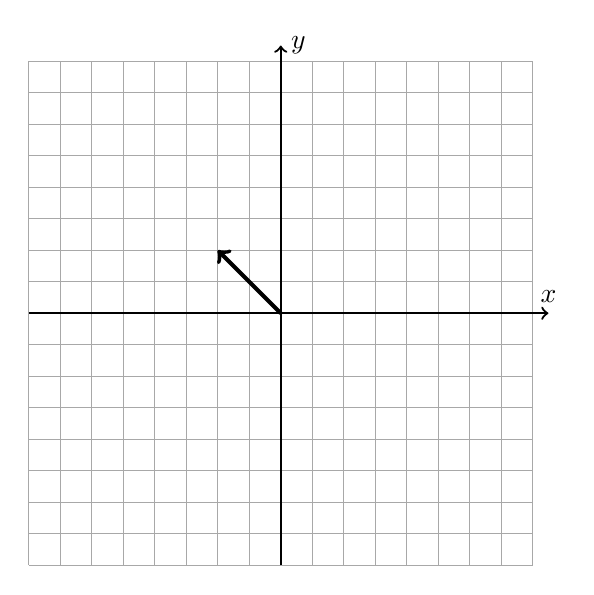
\begin{tikzpicture}[scale=0.8]
        \draw[white!66!black,step=0.50cm] (-4,-4) grid (4,4);
        \draw[thick,->] (-4,0) -- (4.25,0) node[anchor=south] {$x$};
        \draw[thick,->] (0,-4) -- (0,4.25) node[anchor=west] {$y$};
        \draw[line width=1.5pt,->] (0,0) -- ++(-1,1);
    \end{tikzpicture}
    \end{center}
    Choose the option that shows vector $-3\vec{\mathbf{A}}$.
    \begin{multicols}{2}
    \begin{choices}
        \AMCboxDimensions{down=-1.5cm}
        \wrongchoice{
            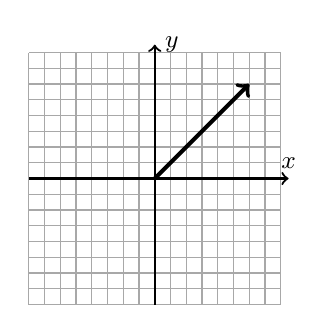
\begin{tikzpicture}[scale=0.4,font=\small]
                \draw[white!66!black,step=0.50cm] (-4,-4) grid (4,4);
                \draw[thick,->] (-4,0) -- (4.25,0) node[anchor=south] {$x$};
                \draw[thick,->] (0,-4) -- (0,4.25) node[anchor=west] {$y$};
                \draw[line width=1.5pt,->] (0,0) -- ++(3,3);
            \end{tikzpicture}
        }
        \wrongchoice{
            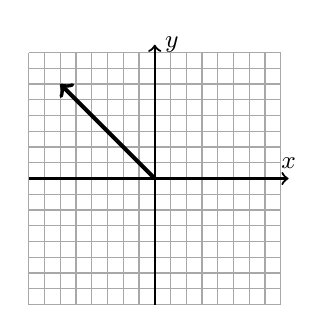
\begin{tikzpicture}[scale=0.4,font=\small]
                \draw[white!66!black,step=0.50cm] (-4,-4) grid (4,4);
                \draw[thick,->] (-4,0) -- (4.25,0) node[anchor=south] {$x$};
                \draw[thick,->] (0,-4) -- (0,4.25) node[anchor=west] {$y$};
                \draw[line width=1.5pt,->] (0,0) -- ++(-3,3);
            \end{tikzpicture}
        }
        \correctchoice{
            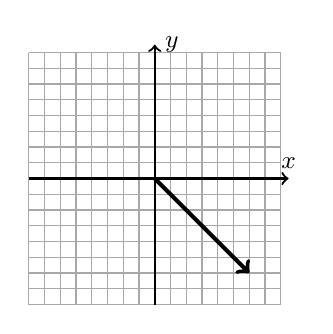
\begin{tikzpicture}[scale=0.4,font=\small]
                \draw[white!66!black,step=0.50cm] (-4,-4) grid (4,4);
                \draw[thick,->] (-4,0) -- (4.25,0) node[anchor=south] {$x$};
                \draw[thick,->] (0,-4) -- (0,4.25) node[anchor=west] {$y$};
                \draw[line width=1.5pt,->] (0,0) -- ++(3,-3);
            \end{tikzpicture}
        }
        \wrongchoice{
            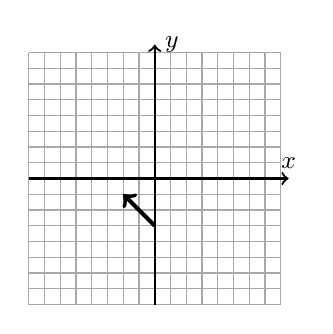
\begin{tikzpicture}[scale=0.4,font=\small]
                \draw[white!66!black,step=0.50cm] (-4,-4) grid (4,4);
                \draw[thick,->] (-4,0) -- (4.25,0) node[anchor=south] {$x$};
                \draw[thick,->] (0,-4) -- (0,4.25) node[anchor=west] {$y$};
                \draw[line width=1.5pt,->] (0,-1.5) -- ++(-1,1);
            \end{tikzpicture}
        }
        \wrongchoice{
            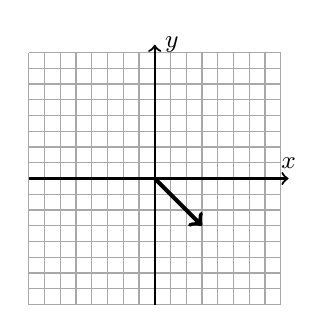
\begin{tikzpicture}[scale=0.4,font=\small]
                \draw[white!66!black,step=0.50cm] (-4,-4) grid (4,4);
                \draw[thick,->] (-4,0) -- (4.25,0) node[anchor=south] {$x$};
                \draw[thick,->] (0,-4) -- (0,4.25) node[anchor=west] {$y$};
                \draw[line width=1.5pt,->] (0,0) -- ++(1.5,-1.5);
            \end{tikzpicture}
        }
    \end{choices}
    \end{multicols}
\end{question}
}

\element{vectors}{
\begin{question}{vectors-q12}
    The figure below shows vectors $\vec{\mathbf{C}}$ and $\vec{\mathbf{A}}$.
    \begin{center}
    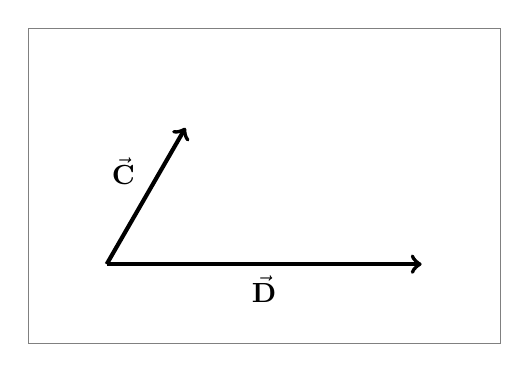
\begin{tikzpicture}
        \draw[help lines] ( -1,-1) rectangle (5,3);
        \draw[line width=1.5pt,->] (0,0) -- (60:2) node[pos=0.5,anchor=south east] {$\vec{\mathbf{C}}$};
        \draw[line width=1.5pt,->] (0,0) -- (0:4) node[pos=0.5,anchor=north] {$\vec{\mathbf{D}}$};
    \end{tikzpicture}
    \end{center}
    Which option is the best interpretation of the cross product
        $\left(\vec{\mathbf{C}}\times\vec{\mathbf{D}}\right)$.
    \begin{choices}
        \wrongchoice{A vector between $\vec{\mathbf{C}}$ and $\vec{\mathbf{D}}$ pointing up to the right.}
        \wrongchoice{A vector perpendicular to both vectors with a direction out of the page.}
        \wrongchoice{The magnitude of a vector between $\vec{\mathbf{C}}$ and $\vec{\mathbf{D}}$ pointing up to the right.}
        \wrongchoice{A quantity in the clock-wise direction.}
      \correctchoice{A vector perpendicular to both vectors with a direction into the page.}
    \end{choices}
\end{question}
}

\element{vectors}{
\begin{question}{vectors-q13}
    The figure below shows vectors $\vec{\mathbf{A}}$ and $\vec{\mathbf{B}}$.
    \begin{center}
    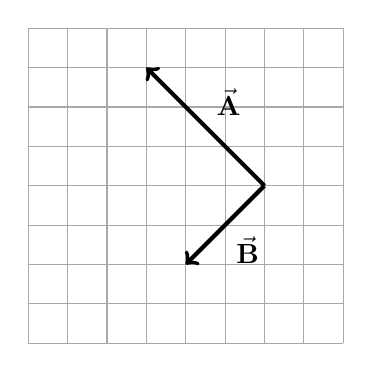
\begin{tikzpicture}
        \draw[white!66!black,step=0.50cm] (0,0) grid (4,4);
        \draw[line width=1.5pt,->] (3,2) -- ++(-1.5,1.5) node[pos=0.5,anchor=south west] {$\vec{\mathbf{A}}$};
        \draw[line width=1.5pt,->] (3,2) -- ++(-1,-1) node[pos=0.5,anchor=north west] {$\vec{\mathbf{B}}$};
    \end{tikzpicture}
    \end{center}
    Choose the option that shows the vector difference $\vec{\mathbf{A}}-\vec{\mathbf{B}}$.
    \begin{multicols}{2}
    \begin{choices}
        \AMCboxDimensions{down=-0.8cm}
        \wrongchoice{
            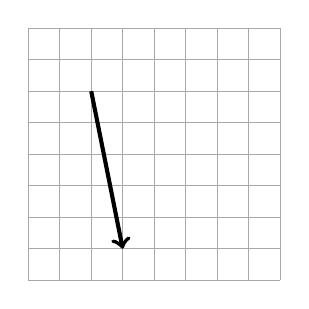
\begin{tikzpicture}[scale=0.8]
                \draw[white!66!black,step=0.50cm] (0,0) grid (4,4);
                \draw[line width=1.5pt,->] (1,3) -- ++(0.5,-2.5);
            \end{tikzpicture}
        }
        \wrongchoice{
            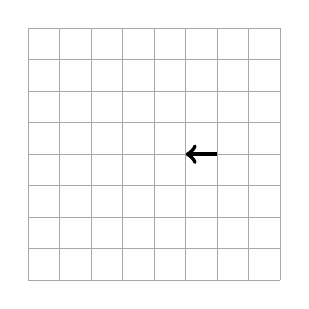
\begin{tikzpicture}[scale=0.8]
                \draw[white!66!black,step=0.50cm] (0,0) grid (4,4);
                \draw[line width=1.5pt,->] (3,2) -- ++(-0.5,0);
            \end{tikzpicture}
        }
        \wrongchoice{
            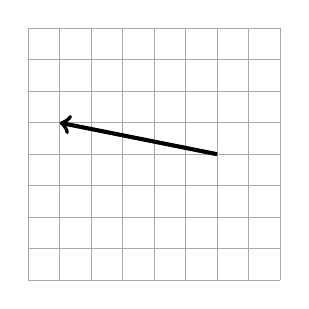
\begin{tikzpicture}[scale=0.8]
                \draw[white!66!black,step=0.50cm] (0,0) grid (4,4);
                \draw[line width=1.5pt,->] (3,2) -- ++(-2.5,0.5);
            \end{tikzpicture}
        }
        \wrongchoice{
            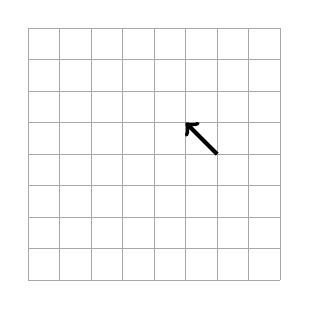
\begin{tikzpicture}[scale=0.8]
                \draw[white!66!black,step=0.50cm] (0,0) grid (4,4);
                \draw[line width=1.5pt,->] (3,2) -- ++(-0.5,0.5);
            \end{tikzpicture}
        }
        \correctchoice{
            \begin{tikzpicture}[scale=0.8]
                \draw[white!66!black,step=0.50cm] (0,0) grid (4,4);
                \draw[line width=1.5pt,->] (2.5,1) -- ++(-0.5,2.5);
            \end{tikzpicture}
        }
    \end{choices}
    \end{multicols}
\end{question}
}

\element{vectors}{
\begin{question}{vectors-q14}
    The figure below shows vector $\vec{\mathbf{A}}$ that forms an angle $\phi$ with the vertical axis.
    \begin{center}
    \begin{tikzpicture}
        %\draw[white] (-0.5,-0.2) rectangle (4.5,4.5);
        %\draw[white!66!black,step=0.5cm] (0,0) grid (4,4);
        \draw[thick,->] (-0.25,0) -- (4.25,0) node[anchor=south] {$x$};
        \draw[thick,->] (0,-0.25) -- (0,4.25) node[anchor=west] {$y$};
        \draw[line width=2pt,->] (0,0) -- (53:5) node[pos=0.5,anchor=north west] {$\vec{\mathbf{A}}$};
        \draw[<->] (0,3) arc (90:53:3) node[anchor=south,pos=0.5] {$\phi$};
    \end{tikzpicture}
    \end{center}
    $\left|\vec{\mathbf{A}}\right|$ is the magnitude of vector $\vec{\mathbf{A}}$.
    Which option shows the magnitude of the $x$-component of vector $\vec{\mathbf{A}}$, (\emph{i.e.} $\vec{\mathbf{A}_x}$)?
    \begin{multicols}{2}
    \begin{choices}
        \wrongchoice{$\left|\vec{\mathbf{A}_x}\right| = \left|\vec{\mathbf{A}}\right| \tan\phi$}
        \wrongchoice{$\left|\vec{\mathbf{A}_x}\right| = \dfrac{\left|\vec{\mathbf{A}}\right|}{\cos\phi}$}
      \correctchoice{$\left|\vec{\mathbf{A}_x}\right| = \left|\vec{\mathbf{A}}\right| \sin\phi$}
        \wrongchoice{$\left|\vec{\mathbf{A}_x}\right| = \left|\vec{\mathbf{A}}\right| \cos\phi$}
        \wrongchoice{$\left|\vec{\mathbf{A}_x}\right| = \dfrac{\left|\vec{\mathbf{A}}\right|}{\sin\phi}$}
    \end{choices}
    \end{multicols}
\end{question}
}

\element{vectors}{
\begin{question}{vectors-q15}
    Consider the vector $\vec{\mathbf{A}} = 1\hat{\imath} + 3\hat{\jmath}$ and the vector $\vec{\mathbf{B}}=5\hat{\imath}$.
    Which option is the cross product $\left(\vec{\mathbf{A}}\times\vec{\mathbf{B}}\right)$?
    \begin{multicols}{2}
    \begin{choices}
      \correctchoice{$-15\hat{k}$}
        \wrongchoice{$5\hat{\imath} + 15\hat{k}$}
        \wrongchoice{$5\hat{\imath} + 3\hat{k}$}
        \wrongchoice{$15\hat{k}$}
        \wrongchoice{$6\hat{\imath} + 3\hat{k}$}
    \end{choices}
    \end{multicols}
\end{question}
}

\element{vectors}{
\begin{question}{vectors-q16}
    The figure below shows vectors $\vec{\mathbf{A}}$ and $\vec{\mathbf{B}}$ that have the same magnitude. 
    \begin{center}
    \begin{tikzpicture}
        \draw[white!66!black,step=0.50cm] (-3,-1) grid (4,3);
        \draw[line width=1.5pt,->] (0,0) -- (0:3) node[pos=0.5,anchor=north] {$\vec{\mathbf{A}}$};
        \draw[line width=1.5pt,->] (0,0) -- (143:3) node[pos=0.5,anchor=north east] {$\vec{\mathbf{B}}$};
    \end{tikzpicture}
    \end{center}
    Which of the following statements about the magnitude of the vector sum of these two vectors is true?
    \begin{choices}
        \wrongchoice{The magnitude of the vector sum is greater than the magnitude of vector, and it is demonstrated by the direct application of the Pythagorean theorem.}
      \correctchoice{The magnitude of the vector sum is smaller than the magnitude of vector, because if we do the graphical addition of the two vectors we note that the vector sum is smaller.}
        \wrongchoice{The magnitude of the vector sum is greater than the magnitude of vector, because the addition of two vectors always gives a resultant vector with a greater magnitude than the vectors that are added up.}
        \wrongchoice{The magnitude of the vector sum is equal to the magnitude of vector, and it is demonstrated by the direct application of the Pythagorean theorem.}
        \wrongchoice{The magnitude of the vector sum is greater than the magnitude of vector, because the distance between the tips of the arrows is longer than the magnitude of vector.}
    \end{choices}
\end{question}
}

\element{vectors}{
\begin{question}{vectors-q17}
    Consider the vector $\vec{\mathbf{A}} = 3\hat{\imath} + 4\hat{\jmath}$.
    Which option shows the direction of this vector as measured from the positive $x$-direction?
    \begin{multicols}{2}
    \begin{choices}
        \wrongchoice{\ang{126.87}}
      \correctchoice{\ang{53.13}}
        \wrongchoice{\ang{143.13}}
        \wrongchoice{\ang{135}}
        \wrongchoice{\ang{-53.13}}
    \end{choices}
    \end{multicols}
\end{question}
}

\element{vectors}{
\begin{question}{vectors-q18}
    The figure below shows vectors $\vec{\mathbf{A}}$ and $\vec{\mathbf{B}}$ that forms an angle $\theta$.
    \begin{center}
    \begin{tikzpicture}
        \draw[help lines] ( -1,-1) rectangle (5,3);
        \draw[line width=1.5pt,->] (0,0) -- (60:2) node[pos=0.5,anchor=south east] {$\vec{\mathbf{A}}$};
        \draw[line width=1.5pt,->] (0,0) -- (0:4) node[pos=0.5,anchor=north] {$\vec{\mathbf{B}}$};
        \draw[<->] (1,0) arc (0:59:1) node[pos=0.5,anchor=west] {$\theta$};
    \end{tikzpicture}
    \end{center}
    $\left|\vec{\mathbf{A}}\right|$ is the magnitude of vector $\vec{\mathbf{A}}$ and $\left|\vec{\mathbf{B}}\right|$ is the magnitude of vector $\vec{\mathbf{B}}$.
    Which option is the magnitude of the cross product $\left(\vec{\mathbf{A}}\times\vec{\mathbf{B}}\right)$?
    \begin{multicols}{2}
    \begin{choices}
        \wrongchoice{$\left|\vec{\mathbf{A}}\right| \cos\theta \left|\vec{\mathbf{B}}\right| \sin\theta$}
        \wrongchoice{$\left|\vec{\mathbf{A}}\right| \left|\vec{\mathbf{B}}\right|$}
        \wrongchoice{$\left|\vec{\mathbf{A}}\right| \left|\vec{\mathbf{B}}\right| \sin\left(\ang{90}-\theta\right)$}
      \correctchoice{$\left|\vec{\mathbf{A}}\right| \left|\vec{\mathbf{B}}\right| \sin\theta$}
        \wrongchoice{$\left|\vec{\mathbf{A}}\right| \left|\vec{\mathbf{B}}\right| \cos\theta$}
    \end{choices}
    \end{multicols}
\end{question}
}

\element{vectors}{
\begin{question}{vectors-q19}
    The figure below shows vectors $\vec{\mathbf{A}}$ and $\vec{\mathbf{B}}$.
    \begin{center}
    \begin{tikzpicture}
        \draw[white!66!black,step=0.50cm] (0,0) grid (4,4);
        \draw[line width=1.5pt,->] (+2.5,3) -- ++(-1.5,0) node[pos=0.5,anchor=south] {$\vec{\mathbf{A}}$};
        \draw[line width=1.5pt,->] (+0.5,1) -- ++(2.5,0) node[pos=0.5,anchor=north] {$\vec{\mathbf{B}}$};
    \end{tikzpicture}
    \end{center}
    Choose the option that shows the vector difference $\vec{\mathbf{A}}-\vec{\mathbf{B}}$.
    \begin{multicols}{2}
    \begin{choices}
        \AMCboxDimensions{down=-0.6cm}
        \wrongchoice{
            \begin{tikzpicture}[scale=0.8]
                \draw[white!66!black,step=0.50cm] (0,0) grid (4,2);
                \draw[line width=1.5pt,->] (0.5,1) -- (2.5,1);
            \end{tikzpicture}
        }
        \wrongchoice{
            \begin{tikzpicture}[scale=0.8]
                \draw[white!66!black,step=0.50cm] (0,0) grid (4,2);
                \draw[line width=1.5pt,->] (0.5,1) -- (1.5,1);
            \end{tikzpicture}
        }
        \wrongchoice{
            \begin{tikzpicture}[scale=0.8]
                \draw[white!66!black,step=0.50cm] (0,0) grid (4,2);
                \draw[line width=1.5pt,<-] (0.5,1) -- (1.5,1);
            \end{tikzpicture}
        }
        \wrongchoice{
            \begin{tikzpicture}[scale=0.8]
                \draw[white!66!black,step=0.50cm] (0,0) grid (4,2);
                \draw[line width=1.5pt,->] (0,1) -- (4,1);
            \end{tikzpicture}
        }
        \correctchoice{
            \begin{tikzpicture}[scale=0.8]
                \draw[white!66!black,step=0.50cm] (0,0) grid (4,2);
                \draw[line width=1.5pt,<-] (0,1) -- (4,1);
            \end{tikzpicture}
        }
    \end{choices}
    \end{multicols}
\end{question}
}

\element{vectors}{
\begin{question}{vectors-q20}
    Consider the vector $\vec{\mathbf{A}} = 2\hat{\imath} + 2\hat{\jmath}$.
    Which option shows the magnitude of this vector?
    \begin{multicols}{2}
    \begin{choices}
        \wrongchoice{$2$}
      \correctchoice{$\sqrt{8}$} %% Also: 2\sqrt{2}
        \wrongchoice{$4$}
        \wrongchoice{$\dfrac{2}{\sqrt{8}}\hat{\imath} + \dfrac{2}{\sqrt{8}}\hat{\jmath}$}
        \wrongchoice{$8$}
    \end{choices}
    \end{multicols}
\end{question}
}


\endinput


